\documentclass[11pt,a4paper]{article}
\usepackage[margin=2.5cm]{geometry}
\usepackage{hyperref}
\usepackage{amsmath,amssymb}
\usepackage{graphicx}
\usepackage{enumitem}
\usepackage{booktabs}
\usepackage{xcolor}
\usepackage{tcolorbox}
\usepackage{tikz}
\usetikzlibrary{arrows.meta, positioning, shapes.geometric}

\hypersetup{colorlinks=true, linkcolor=blue, urlcolor=blue, citecolor=blue}

\title{%
  \textbf{Objective 1 --- Explained From Scratch} \\[6pt]
  \large A Beginner-Friendly Guide to the Memo
}
\author{Youssef --- PFE Research Project}
\date{February 21, 2026}

\begin{document}
\maketitle

\begin{tcolorbox}[colback=green!5, colframe=green!50!black, title=What is this document?]
This document explains \textbf{every concept} in Meeting Memo~\#2 in plain
language.  If you read that memo and thought ``I don't understand a single
word,'' this is for you.  No prior knowledge of offshore engineering, soil
mechanics, or AI is assumed.  Each section below matches a section of the memo.
\end{tcolorbox}

\tableofcontents
\newpage

% ====================================================================
%  PART A  ---  THE REAL-WORLD PROBLEM
% ====================================================================
\part{The Real-World Problem}
% ====================================================================

% ====================================================================
\section{What Is an Offshore Wind Turbine (OWT)?}
% ====================================================================

A wind turbine converts wind into electricity.  An \textbf{offshore} wind
turbine is one built in the sea, usually several kilometres from the coast,
because ocean wind is stronger and steadier than onshore wind.

Modern offshore turbines are \textbf{enormous} --- over 200~metres tall
(taller than the Eiffel Tower) and can produce 10--16~MW of power, enough
to supply roughly 10\,000 homes.

% ====================================================================
\section{What Holds the Turbine Up?  The Monopile}
% ====================================================================

Over 60\% of offshore turbines worldwide stand on a \textbf{monopile} --- a
single giant steel cylinder hammered 25--60~metres into the seabed.  Think of
sticking a huge metal straw into wet sand.

\begin{center}
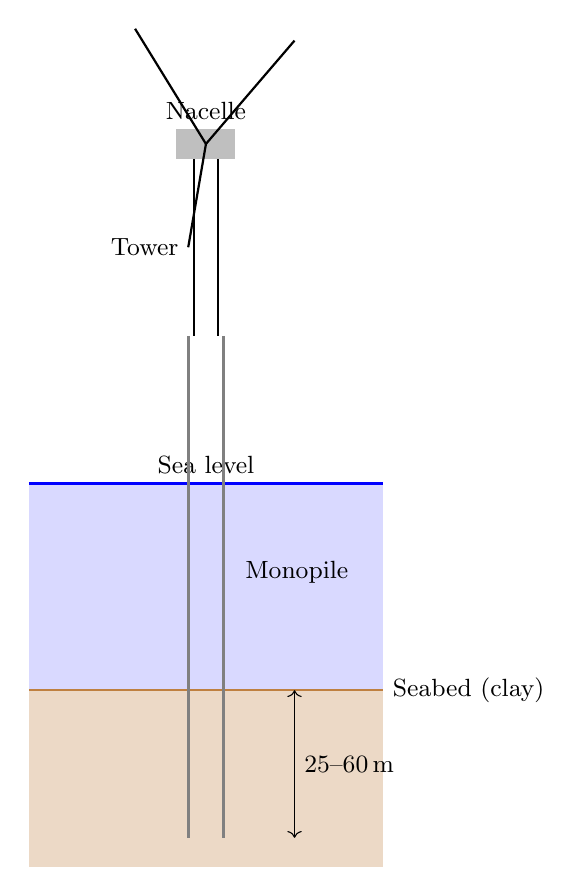
\begin{tikzpicture}[scale=0.75]
  % Sea
  \fill[blue!15] (-3,-0.5) rectangle (3,-4);
  \draw[thick, blue] (-3,-0.5) -- (3,-0.5);
  \node[above] at (0,-0.5) {\small Sea level};

  % Seabed
  \fill[brown!30] (-3,-4) rectangle (3,-7);
  \draw[thick, brown] (-3,-4) -- (3,-4);
  \node[right] at (3,-4) {\small Seabed (clay)};

  % Monopile
  \draw[very thick, gray] (-0.3,2) -- (-0.3,-6.5);
  \draw[very thick, gray] (0.3,2) -- (0.3,-6.5);
  \node[right] at (0.5,-2) {\small Monopile};

  % Tower + nacelle
  \draw[thick] (-0.2,2) -- (-0.2,5);
  \draw[thick] (0.2,2) -- (0.2,5);
  \fill[gray!50] (-0.5,5) rectangle (0.5,5.5);
  \node[above] at (0,5.5) {\small Nacelle};

  % Blades
  \draw[thick] (0,5.25) -- (1.5,7);
  \draw[thick] (0,5.25) -- (-1.2,7.2);
  \draw[thick] (0,5.25) -- (-0.3,3.5);
  \node[left] at (-0.3,3.5) {\small Tower};

  % Depth label
  \draw[<->] (1.5,-4) -- (1.5,-6.5);
  \node[right] at (1.5,-5.25) {\small 25--60\,m};
\end{tikzpicture}
\end{center}

The monopile transfers every force (wind pushing the blades, waves hitting the
tower) down into the soil.  The soil \textbf{pushes back} and keeps the pile in
place.  That push-back is what engineers call \textbf{stiffness}.

% ====================================================================
\section{What Is ``Stiffness''?}
% ====================================================================

Imagine pushing a pencil into a block of cheese vs.\ a block of concrete:
\begin{itemize}[noitemsep]
  \item \textbf{Cheese} = low stiffness --- the pencil moves easily.
  \item \textbf{Concrete} = high stiffness --- the pencil barely moves.
\end{itemize}

For a monopile, the \textbf{soil stiffness} decides how much the pile tilts
or sways.  Higher stiffness = less movement = safer turbine.

The memo mentions a ``3DOF stiffness matrix.''  That's simply three types of
stiffness bundled together:

\begin{center}
\begin{tabular}{clp{6.5cm}}
\toprule
\textbf{Symbol} & \textbf{Name} & \textbf{Plain English} \\
\midrule
$K_L$     & Lateral     & Resistance to sideways sliding. \\
$K_R$     & Rotational  & Resistance to tilting (the most important one). \\
$K_{LR}$  & Coupled     & How sliding and tilting affect each other. \\
\bottomrule
\end{tabular}
\end{center}

``3DOF'' stands for ``3 Degrees of Freedom'' --- three independent ways the pile
can move (slide, tilt, and a mix of both).

% ====================================================================
\section{What Is ``Natural Frequency'' ($f_0$)?}
\label{sec:f0}
% ====================================================================

Every object has a rate at which it ``wants'' to vibrate --- its
\textbf{natural frequency}.

\begin{itemize}[noitemsep]
  \item A guitar string vibrates at a specific pitch when plucked.
  \item A playground swing has a natural frequency --- push it at that rhythm
        and it goes higher and higher.
\end{itemize}

An offshore wind turbine also has a natural frequency ($f_0$), typically
\textbf{0.2--0.35~Hz} (one vibration every 3--5 seconds).  It depends
heavily on how stiff the foundation soil is.

\begin{tcolorbox}[colback=red!5, colframe=red!50!black, title=Why $f_0$ matters: Resonance]
The spinning blades create vibrations at frequencies called $f_{1P}$ and
$f_{3P}$.  Engineers design the turbine so $f_0$ sits \textbf{between} these
blade frequencies (the ``soft-stiff'' design).  The margin is only about
\textbf{10\%}.

If $f_0$ shifts by just 5--10\%, it can match a blade frequency, causing
\textbf{resonance} --- vibrations amplify 150--300\%.  For a 200-metre tower,
that can be catastrophic.

\medskip
\textit{Analogy:} Pushing a swing at exactly the right rhythm makes it fly
dangerously high.  That's resonance.
\end{tcolorbox}

% ====================================================================
\section{The Typhoon Problem}
% ====================================================================

Typhoons (the Asian name for hurricanes) bring extreme wind and waves.  This
project focuses on \textbf{Shenzhen, Guangdong Province, China} --- the
world's most active typhoon corridor.

When a typhoon hits, the extreme back-and-forth forces do something dangerous
to the clay soil around the monopile:

\begin{center}
  \textbf{The soil gets softer.}
\end{center}

This is called \textbf{stiffness degradation}.  The clay loses its ability to
push back against the pile.

Engineers measure degradation with the ratio $G/G_{\max}$:
\begin{itemize}[noitemsep]
  \item $G_{\max}$ = original (maximum) soil stiffness.
  \item $G$ = current stiffness after the storm.
  \item $G/G_{\max} = 0.7$ means 30\% of the stiffness is gone.
\end{itemize}

% ====================================================================
\section{The Correlation Chain (Core of Objective 1)}
\label{sec:chain}
% ====================================================================

Here is the chain reaction that Objective~1 aims to capture:

\begin{center}
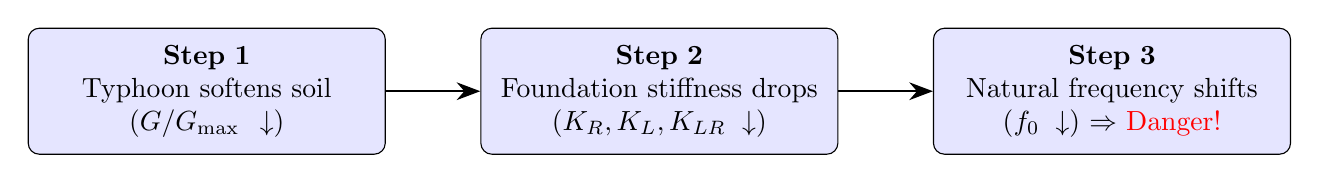
\begin{tikzpicture}[
  node distance=1.2cm,
  block/.style={rectangle, draw, fill=blue!10, text width=4.3cm,
                text centered, rounded corners, minimum height=1.6cm},
  arrow/.style={-{Stealth[length=3mm]}, thick}
]
  \node[block] (soil) {%
    \textbf{Step 1} \\
    Typhoon softens soil \\
    ($G/G_{\max} \downarrow$)
  };
  \node[block, right=of soil] (found) {%
    \textbf{Step 2} \\
    Foundation stiffness drops \\
    ($K_R, K_L, K_{LR} \downarrow$)
  };
  \node[block, right=of found] (freq) {%
    \textbf{Step 3} \\
    Natural frequency shifts \\
    ($f_0 \downarrow$) $\Rightarrow$ \textcolor{red}{Danger!}
  };
  \draw[arrow] (soil) -- (found);
  \draw[arrow] (found) -- (freq);
\end{tikzpicture}
\end{center}

\textbf{The problem today:} Engineers need two separate, expensive computer
simulations to predict this chain.  Each takes 20--32 hours.  Real-time
monitoring during a typhoon is therefore impossible.

\textbf{Objective~1's solution:} Build a \textit{single AI model} that
captures the entire chain in one shot, in seconds.


% ====================================================================
%  PART B  ---  THE AI MODEL (WHAT IS IT?)
% ====================================================================
\newpage
\part{The AI Model --- What Is It?}
% ====================================================================

% ====================================================================
\section{What Is a ``Transformer''?}
% ====================================================================

A \textbf{transformer} is a type of AI architecture --- the same family of
technology behind ChatGPT and Google Translate.

Three key properties:
\begin{enumerate}
  \item \textbf{Processes sequences:} Takes a sequence of inputs (words in a
        sentence, or load measurements over time) and produces a sequence of
        outputs (a translation, or predicted frequencies over time).
  \item \textbf{Attention mechanism:} The transformer can ``pay attention'' to
        the most important parts of the input.  In our case, it learns that
        \textit{peak typhoon loads} relate to \textit{large stiffness drops}.
  \item \textbf{Very flexible:} It can learn complex, nonlinear relationships
        from data.
\end{enumerate}

\begin{tcolorbox}[colback=yellow!5, colframe=yellow!50!black, title=Analogy]
Think of the transformer as a smart student reading a textbook (the input
data).  The attention mechanism is a highlighter --- it marks the important
sentences.  After reading, the student answers questions (makes predictions)
based on what they highlighted.
\end{tcolorbox}

% ====================================================================
\section{What Does ``Physics-Informed'' Mean?}
% ====================================================================

Normal AI learns \textit{only from data}.  This is dangerous in engineering
because it might predict impossible things (e.g., soil getting \textit{stiffer}
during a storm --- which violates physics).

A \textbf{physics-informed} AI is forced to obey physical laws during
training.  Specifically:

\begin{enumerate}
  \item \textbf{Law of Thermodynamics \#1 (LoT1)} --- energy conservation.
        The predicted stiffness values must be consistent with the natural
        frequency.  You can't have high stiffness but low frequency.

  \item \textbf{Law of Thermodynamics \#2 (LoT2)} --- entropy always
        increases (``things only get worse'').  During a storm, stiffness can
        only \textit{decrease}.  No magical soil ``gains.''
\end{enumerate}

These rules are enforced through the \textbf{loss function}
(Section~\ref{sec:loss}).

% ====================================================================
\section{What Is ``Explainable AI'' (XAI)?}
% ====================================================================

Most AI is a ``black box'' --- it gives an answer but can't explain \textit{why}.
This is a problem because engineers must \textbf{trust} the model before
using it on real multi-million-dollar turbines.

\textbf{XAI} means we can open the black box.  In our transformer, this is
done through \textbf{attention maps}: heat maps showing which inputs the model
focused on for each prediction.

% ====================================================================
\section{What Is ``Self-Calibrating''?}
% ====================================================================

Traditionally, every new site (different soil, different pile) requires an
expert to manually adjust (``calibrate'') model parameters.

\textbf{Self-calibrating} means the AI does this automatically: you feed in
basic soil and pile properties, and it figures out the right internal
parameters by itself.  This is the job of the \textbf{slot-attention module}
(Section~\ref{sec:slots}).


% ====================================================================
%  PART C  ---  THE ARCHITECTURE, PIECE BY PIECE
% ====================================================================
\newpage
\part{The Architecture --- Piece by Piece}

These sections explain each of the \textbf{6 Steps} in the memo's
implementation plan.
% ====================================================================

% ====================================================================
\section{Step 1 --- The Physics Equation (TIM Formulation)}
\label{sec:TIM}
% ====================================================================

TIM stands for \textbf{Thermodynamically consistent Inertial Macroelement}.
It is a single equation that describes how foundation stiffness decreases
as loads grow:

\begin{equation*}
  \underbrace{H_{ij}(t)}_{\text{current stiffness}}
  \;=\;
  \underbrace{H^0_{ij}}_{\text{starting stiffness}}
  \;-\;
  \sum_{n=1}^{20}
  \underbrace{w_n(t)}_{\substack{\text{how ``activated''} \\
                                   \text{is drop } n\text{?}}}
  \;\cdot\;
  \underbrace{H^n_{ij}}_{\substack{\text{size of} \\
                                    \text{drop } n}}
\end{equation*}

\textbf{In plain English:}
\begin{itemize}[noitemsep]
  \item You start with an initial stiffness $H^0$.
  \item As loads increase, stiffness drops in \textbf{20 small steps}.
  \item Each step~$n$ has a \textit{size} ($H^n$) and a \textit{trigger}
        ($w_n$).
  \item $w_n(t)$ is a number between 0 and 1.  It starts at~0 (drop hasn't
        happened) and smoothly rises to~1 (drop fully activated) as loads
        grow.
  \item The smooth transition uses a \textbf{sigmoid function} --- an
        S-shaped curve going from 0 to 1.
\end{itemize}

\begin{tcolorbox}[colback=yellow!5, colframe=yellow!50!black, title=Analogy]
Imagine a stack of 20 ice cubes supporting a weight.  As you heat them
(= apply loads), they melt one by one.  Each melting is one ``stiffness
drop.''  Total support = original support minus all the melted cubes.
\end{tcolorbox}

\textbf{Why 20?}  The TIM uses 20 ``yield surfaces'' --- 20 damage levels
from minor to severe.

\medskip
The memo also mentions \textbf{physics constraints} embedded in the model:
\begin{center}
\begin{tabular}{clp{7cm}}
\toprule
\textbf{Rule} & \textbf{From} & \textbf{What it says} \\
\midrule
$\mathcal{L}_{\text{freq}}$ & LoT1 &
  Predicted stiffness must be consistent with predicted frequency. \\
$\mathcal{L}_{\text{1mon}}, \mathcal{L}_{\text{2mon}}$ & LoT2 &
  Stiffness can only decrease; drops activate in order. \\
$\mathcal{L}_{\text{pos}}$ & LoT2 &
  Stiffness must always stay positive (can't go below zero). \\
\bottomrule
\end{tabular}
\end{center}

These are penalty terms added to the loss function (see Section~\ref{sec:loss}).

% ====================================================================
\section{Step 2 --- Preparing the Training Data}
\label{sec:data}
% ====================================================================

AI learns by example.  You show it many ``input $\to$ correct answer'' pairs
and it discovers the pattern.

\begin{center}
\begin{tabular}{lp{6.5cm}}
\toprule
\textbf{Input (what we give)} & \textbf{Output (what it should predict)} \\
\midrule
Soil properties ($G_{\max}$, $s_u$) & Stiffness evolution $H(t)$ \\
Pile properties ($D$, $L$, $EI$) & Natural frequency evolution $f_0(t)$ \\
Typhoon load sequence & \\
\bottomrule
\end{tabular}
\end{center}

\textbf{Where does the data come from?}
\begin{enumerate}
  \item \textbf{Computer simulations (FEM) --- $\sim$300 cases:}
    \begin{itemize}[noitemsep]
      \item Run in a free engineering software called \textbf{OpenSees}.
      \item Each simulation models a specific combination of soil, pile, and
            typhoon conditions and takes 20--32 hours.
      \item Outputs: how stiffness changes over time during the typhoon.
    \end{itemize}

  \item \textbf{Lab experiments --- $\sim$30 cases:}
    \begin{itemize}[noitemsep]
      \item 1:50 scale physical models of turbines built in real Shenzhen clay.
      \item Hit with a hammer at each loading stage to measure the real
            frequency ($f_0$).
      \item Outputs: measured load-vs-frequency pairs.
    \end{itemize}
\end{enumerate}

The memo shows a parameter table covering turbine size (5--16~MW), pile
diameter (4--10~m), clay strength (20--130~kPa), typhoon severity
(5/10/50-year return), etc.  This defines the ``universe'' of conditions the
AI must learn to handle.

% ====================================================================
\section{Step 3 --- The Self-Calibration Module (Slot Attention)}
\label{sec:slots}
% ====================================================================

This module replaces manual calibration.  It uses a technique called
\textbf{slot attention} (Locatello et al., 2020).

\subsection{What is a ``slot''?}

A slot is a small \textbf{learnable memory container} inside the AI.  Each
slot specializes in one specific task.

In our model there are \textbf{21~slots}:
\begin{itemize}[noitemsep]
  \item \textbf{Slot~1} --- learns to calculate the initial stiffness $H^0$
        from soil/pile properties.
  \item \textbf{Slots 2--21} --- each learns one of the 20 stiffness drops
        ($H^n$ and its trigger $w_n$).
\end{itemize}

\subsection{How do the slots work together?}

\begin{enumerate}
  \item \textbf{Cross-attention:} Each slot ``looks at'' the input parameters
        and extracts what \textit{it} needs.

        \textit{Example:} Slot~1 might focus on $G_{\max}$ and pile diameter
        $D$ (which determine initial stiffness), while Slot~15 focuses on
        load intensity (which determines when its drop triggers).

  \item \textbf{Self-attention:} The slots ``talk to each other'' so they
        don't duplicate work --- each one specializes in a distinct drop.

  \item \textbf{MLP decoders:} Small neural networks attached to each slot
        that convert its internal state into actual numbers ($H^0$, $H^n$,
        $w_n$).
\end{enumerate}

\begin{tcolorbox}[colback=yellow!5, colframe=yellow!50!black, title=Analogy]
Imagine 21 specialist doctors examining a patient (the soil/pile data).
Doctor~1 checks baseline health ($H^0$).  Doctors 2--21 each look for a
specific disease (stiffness drop).  They first read the patient's file
(cross-attention), then consult each other to avoid duplicate diagnoses
(self-attention), and finally each writes their report (MLP decoder).
\end{tcolorbox}

\textbf{Jargon decoder:}
\begin{itemize}[noitemsep]
  \item \textbf{Cross-attention} = one set of data (slots) reads another set
        of data (soil/pile inputs).
  \item \textbf{Self-attention} = a set of data reads \textit{itself} to find
        internal relationships.
  \item \textbf{MLP} = Multi-Layer Perceptron, a small feed-forward neural
        network (a few simple layers of math).
\end{itemize}

% ====================================================================
\section{Step 4 --- The Full Transformer Architecture}
\label{sec:transformer}
% ====================================================================

The complete model has two halves --- an \textbf{encoder} and a
\textbf{decoder}.

\subsection{Encoder (the ``reader'')}

\begin{enumerate}[noitemsep]
  \item \textbf{Tokenize} the inputs: turn the soil properties, pile
        properties, and typhoon load sequence into small numerical chunks
        called ``tokens'' (just like how a chatbot splits a sentence into
        words).
  \item Add \textbf{positional encoding}: a label that tells the model the
        \textit{order} of each token (``this load happened at time step~5,
        that one at time step~6'').
  \item Process everything through \textbf{self-attention layers}: the model
        learns which inputs relate to each other.
  \item Feed the result into the \textbf{slot-attention module}
        (Section~\ref{sec:slots}) $\Rightarrow$ outputs the stiffness matrix
        $H(t)$ at every time step.
\end{enumerate}

\subsection{Decoder (the ``writer'')}

\begin{enumerate}[noitemsep]
  \item \textbf{Masked self-attention}: the decoder can only see past and
        present --- never the future.  (You can't use tomorrow's weather to
        predict today's.)
  \item \textbf{Cross-attention}: combines stiffness info from the encoder
        with previous frequency predictions.
  \item \textbf{Feed-forward network + linear layer} $\Rightarrow$ predicts
        the natural frequency $f_0^{\text{OWT}}(t)$ at each time step.
\end{enumerate}

\begin{tcolorbox}[colback=yellow!5, colframe=yellow!50!black, title=Analogy]
\textbf{Encoder} = reading and understanding a book about what happened
during the typhoon. \\
\textbf{Decoder} = writing a prediction report, one chapter (time step) at
a time, based on what was read.
\end{tcolorbox}

% ====================================================================
\section{The Loss Function --- How the AI Learns}
\label{sec:loss}
% ====================================================================

A \textbf{loss function} measures ``how wrong is the AI right now?''  During
training the AI adjusts itself to make this number as small as possible.
Think of it like a golf score --- lower is better.

\subsection{The five components}

\begin{center}
\begin{tabular}{clp{7cm}}
\toprule
\textbf{Symbol} & \textbf{Name} & \textbf{Plain English} \\
\midrule
$\mathcal{L}_{\text{data}}$ & Data loss &
  How far off are predictions from the real data? \\[4pt]
$\mathcal{L}_{\text{freq}}$ & Frequency loss (LoT1) &
  Is predicted frequency consistent with predicted stiffness?
  (energy conservation check) \\[4pt]
$\mathcal{L}_{\text{1mon}}$ & Monotonicity 1 (LoT2) &
  Are drops always increasing?  (drops can't ``un-happen'') \\[4pt]
$\mathcal{L}_{\text{2mon}}$ & Monotonicity 2 (LoT2) &
  Do drops activate in order?  (mild before severe) \\[4pt]
$\mathcal{L}_{\text{pos}}$ & Positivity (LoT2) &
  Is stiffness always $\geq 0$?  (negative stiffness is
  physically impossible) \\
\bottomrule
\end{tabular}
\end{center}

\subsection{The total loss}

\[
  \mathcal{L}_{\text{total}}
  = \underbrace{\alpha}_{\text{weight}} \cdot \mathcal{L}_{\text{data}}
  + \beta \cdot \mathcal{L}_{\text{freq}}
  + \gamma \cdot (\mathcal{L}_{\text{1mon}} + \mathcal{L}_{\text{2mon}})
  + \delta \cdot \mathcal{L}_{\text{pos}}
\]

$\alpha, \beta, \gamma, \delta$ are \textbf{weights} that control how much
the AI ``cares'' about each component.  They are tuned during development.

\begin{tcolorbox}[colback=yellow!5, colframe=yellow!50!black, title=Analogy]
Imagine grading a student's exam.  $\mathcal{L}_{\text{data}}$ checks if the
answers match the answer key.  The physics losses ($\mathcal{L}_{\text{freq}}$,
$\mathcal{L}_{\text{1mon}}$, etc.) check if the student showed correct working
--- even a right answer with wrong reasoning gets penalised.
\end{tcolorbox}

% ====================================================================
\section{Step 5 --- Attention Roll-Out for XAI}
\label{sec:xai}
% ====================================================================

This is the step that \textbf{opens the black box}.

\subsection{What are attention maps?}

The transformer stores which inputs it ``paid attention to'' for every
prediction.  We can visualise this as a \textbf{heat map} --- a coloured grid
where bright = high attention, dark = ignored.

\textbf{What we expect to see:}
\begin{itemize}[noitemsep]
  \item When predicting frequency at the end of a strong typhoon $\Rightarrow$
        high attention on \textbf{peak load} moments.
  \item Slot~1 (initial stiffness) $\Rightarrow$ high attention on
        $G_{\max}$ and pile diameter $D$.
  \item Rotational stiffness $K_R$ $\Rightarrow$ more attention than $K_L$,
        because $K_R$ dominates frequency shifts.
\end{itemize}

If the patterns match physical expectations, the model has \textbf{learned
the right physics} --- not just memorised data.

\subsection{What is attention roll-out?}

A transformer has many layers.  To trace how information flows from the very
first input to the final output, we use \textbf{attention roll-out}:

\begin{enumerate}[noitemsep]
  \item Start at the last layer (closest to the output).
  \item Multiply the attention matrices layer by layer, going backward.
  \item The result is a single \textbf{attribution score} per input, showing
        its total contribution to the final prediction.
\end{enumerate}

This produces a \textbf{bar chart}: each bar = one input (a soil property,
a pile dimension, or a specific moment in the typhoon load history).
Tall bars = most influential inputs.

\begin{tcolorbox}[colback=yellow!5, colframe=yellow!50!black, title=Analogy]
A detective solving a case:
\begin{itemize}[noitemsep]
  \item \textbf{Attention maps} = examining each clue individually.
  \item \textbf{Attention roll-out} = tracing the entire chain of evidence
        from the crime scene to the verdict, showing which clues were
        decisive.
\end{itemize}
\end{tcolorbox}

\textbf{This is how we quantify the correlation chain}
(Section~\ref{sec:chain}):
\begin{itemize}[noitemsep]
  \item High attribution on soil stiffness inputs $\Rightarrow$ confirms the
        soil$\to$foundation link.
  \item High attribution on stiffness tokens $\Rightarrow$ confirms the
        foundation$\to$$f_0$ link.
  \item Together they prove the model has truly captured the full chain.
\end{itemize}

% ====================================================================
\section{Step 6 --- Testing, Validation, and Iteration}
\label{sec:testing}
% ====================================================================

\subsection{Train / test split}

We never test the model on data it learned from (that would be like giving a
student the exam answers beforehand).  Instead:
\begin{itemize}[noitemsep]
  \item \textbf{85\%} of data for training (learning).
  \item \textbf{15\%} for testing (checking it actually learned).
  \item \textbf{3 extra experiments} outside the normal ranges (e.g., bigger
        piles, softer clay) to test ``extrapolation'' --- can the model handle
        situations it has \textit{never seen}?
\end{itemize}

\subsection{Accuracy metrics}

\begin{center}
\begin{tabular}{lp{8.5cm}}
\toprule
\textbf{Metric} & \textbf{Meaning} \\
\midrule
MSE &
  Mean Squared Error --- average of (prediction $-$ truth)$^2$.
  Lower = better. \\[3pt]
$R^2$ &
  R-squared --- how much variation the model explains.
  $R^2 = 1.0$ is perfect, $R^2 = 0$ is useless. \\[3pt]
MAPE &
  Mean Absolute Percentage Error --- average \% difference.
  Target for $f_0$: MAPE $< 1\%$, because even a 10\% shift can be
  catastrophic. \\
\bottomrule
\end{tabular}
\end{center}

\subsection{Validation against reality}

The ultimate check is comparing predictions against:
\begin{enumerate}[noitemsep]
  \item \textbf{Centrifuge experiments} --- lab models spun at
        50$\times$~gravity to simulate real ocean pressures.
  \item \textbf{Field measurements} --- data from an actual 3.6~MW turbine
        during a real typhoon.
  \item \textbf{3~out-of-domain experiments} --- conditions beyond the
        training ranges.
\end{enumerate}

\subsection{Iteration using XAI}

If results aren't good enough, the attention maps guide improvements:
\begin{itemize}[noitemsep]
  \item Low-attention inputs can be pruned (removed).
  \item High-attention load windows get more training data.
  \item Physics losses can be reweighted.
\end{itemize}


% ====================================================================
%  PART D  ---  THE BIG PICTURE
% ====================================================================
\newpage
\part{The Big Picture}
% ====================================================================

% ====================================================================
\section{Summary Table}
% ====================================================================

\begin{center}
\begin{tabular}{cp{10cm}}
\toprule
\textbf{Step} & \textbf{What You Do} \\
\midrule
1 & Learn the TIM physics: how $H_{ij}(t)$ degrades via 20 yield surfaces. \\
2 & Generate training data: $\sim$300 FEM simulations + $\sim$30 experiments. \\
3 & Pre-train the slot-attention module: auto-calibrate $H^0$, $H^n$, $w_n$. \\
4 & Train the full encoder--decoder transformer: loads $\to$ $f_0^{\text{OWT}}$. \\
5 & Run attention roll-out: quantify every link in the correlation chain. \\
6 & Test, validate, iterate using XAI insights. \\
\bottomrule
\end{tabular}
\end{center}

% ====================================================================
\section{Summary in One Paragraph}
% ====================================================================

\begin{tcolorbox}[colback=blue!5, colframe=blue!50!black]
Typhoons soften the clay soil around offshore wind turbine monopile
foundations.  This softening reduces the foundation stiffness, which shifts
the turbine's natural frequency toward dangerous resonance zones.  Currently,
predicting this chain takes expensive simulations too slow for real-time
monitoring.  Objective~1 builds an AI model (a physics-informed XAI
transformer) that learns the entire soil $\to$ foundation $\to$ $f_0$ chain
from data and physics, predicts frequency shifts in seconds, explains its
reasoning via attention maps, and auto-calibrates itself for any soil/pile
configuration.
\end{tcolorbox}

% ====================================================================
\section{Glossary}
% ====================================================================

\begin{center}
\small
\begin{tabular}{lp{9.5cm}}
\toprule
\textbf{Term} & \textbf{Plain English} \\
\midrule
OWT & Offshore Wind Turbine. \\
Monopile & Giant steel tube hammered into the seabed. \\
$f_0$ & Natural frequency --- the rate at which the turbine wants to vibrate. \\
$G/G_{\max}$ & How much soil stiffness remains (1.0 = full, 0.5 = half gone). \\
$K_R, K_L, K_{LR}$ & Foundation stiffness (rotational, lateral, coupled). \\
3DOF & 3 Degrees of Freedom (slide, tilt, coupled). \\
Resonance & Forcing frequency matches natural frequency $\Rightarrow$ huge vibrations. \\
TIM & Thermodynamic Inertial Macroelement --- the physics equation. \\
FEM / OpenSees & Finite Element Method / the software used for detailed simulations. \\
Transformer & AI architecture that processes sequences using attention. \\
Encoder & The part that reads and understands the input. \\
Decoder & The part that generates the output prediction. \\
Slot attention & AI trick where internal ``slots'' each learn a specific task. \\
Cross-attention & One data set reads another data set. \\
Self-attention & Data reads itself to find internal relationships. \\
Masked self-attention & Self-attention that can't look into the future. \\
Positional encoding & Tells the model the order/time of each input. \\
Physics-informed & AI forced to obey physical laws during training. \\
XAI & Explainable AI --- AI whose reasoning can be inspected. \\
Attention map & Heat map showing what the model focused on. \\
Attention roll-out & Tracing attention through all layers for total attribution. \\
Loss function & Score measuring ``how wrong is the AI?'' (lower = better). \\
LoT1 / LoT2 & First / second law of thermodynamics. \\
Sigmoid & S-shaped curve smoothly going from 0 to 1. \\
MLP & Multi-Layer Perceptron --- a small neural network. \\
MSE & Mean Squared Error (accuracy metric). \\
$R^2$ & R-squared --- goodness of fit (1.0 = perfect). \\
MAPE & Mean Absolute Percentage Error. \\
Centrifuge test & Lab test at high gravity to simulate real pressures. \\
\bottomrule
\end{tabular}
\end{center}

\end{document}
